\documentclass{article}
\usepackage{graphicx} % Required for inserting images

\title{ML_Group_Project}
\author{Nilaxy Thirugnanaseelan}
\date{June 2026}

\begin{document}

\section{Evaluation Design}

The evaluation was designed to test whether the Shakespeare-aware system satisfies the assignment requirements for concept explanation, contextual question answering, evidence retrieval, and stylised generation. The final evaluation set contains twelve questions: five instructor-provided questions and seven group-designed questions. These questions cover the four required interaction types and include additional robustness tests such as cross-play comparison, ambiguity handling, and no-good-answer questions.

\subsection{Evaluation Questions}

The instructor questions test core understanding of Macbeth, Hamlet, and Romeo and Juliet. The group-designed questions extend this by testing Lady Macbeth's influence, Juliet's conflict, evidence retrieval, stylised generation, cross-play comparison, and unsupported modern content. This combination allows the evaluation to measure both normal performance and failure behaviour.

\subsection{Scoring Rubric}

Each output was scored from 1 to 5 using five criteria: correctness, grounding, retrieval relevance, usefulness for a beginner, and style quality. Correctness measures factual accuracy. Grounding measures whether the answer is supported by retrieved evidence. Retrieval relevance measures whether the retrieved passages match the question. Usefulness measures whether the answer helps a beginner understand the play. Style quality checks whether stylised responses have a Shakespearean tone while remaining understandable.

\subsection{Evaluation Procedure}

The baseline and RAG systems were evaluated using the same question set. The baseline used the same language model but without retrieved Shakespeare passages. The RAG system embedded the query, retrieved the top relevant chunks, constructed a prompt using the retrieved context, and generated an evidence-grounded answer. The evaluation runner recorded the question, expected focus, system type, retrieved evidence, generated answer, scores, and comments.

\begin{table}[h]
\centering
\caption{Average Evaluation Scores for Baseline and RAG Systems}
\label{tab:average_scores}

\begin{tabular}{|l|c|c|c|}
\hline
\textbf{System} & \textbf{Correctness} & \textbf{Grounding} & \textbf{Usefulness} \\
\hline
Baseline & 2.83 & 1.00 & 2.67 \\
RAG-Based System & 4.83 & 4.83 & 4.00 \\
\hline
\end{tabular}

\end{table}


\begin{figure}[h]
\centering
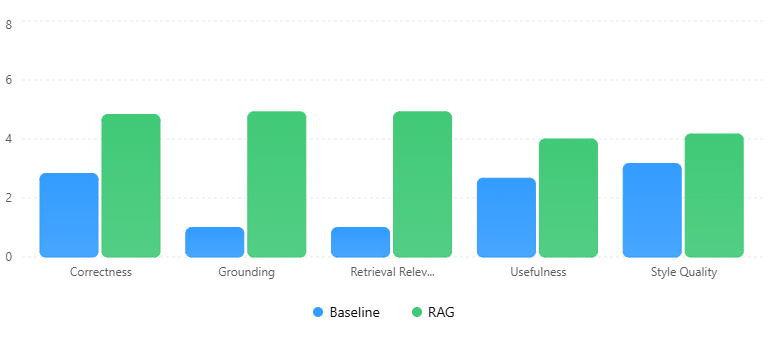
\includegraphics[width=0.48\textwidth]{figures/evaluation_comparison_chart.png}\caption{Baseline and RAG average scores across five evaluation criteria.}
\label{fig}
\end{figure}



\section{Results and Analysis}

\subsection{Baseline versus RAG Comparison}

Table~\ref{tab:average_scores} shows that the RAG-based system performed better than the baseline system across the main evaluation criteria. The baseline achieved an average correctness score of 2.83, grounding score of 1.00, and usefulness score of 2.67. The RAG-based system achieved higher scores of 4.83 for correctness, 4.83 for grounding, and 4.00 for usefulness.

The largest improvement was in grounding because the RAG system retrieved Shakespeare passages and used them as evidence when generating answers. The baseline system sometimes produced fluent and understandable answers, but these answers were often unsupported by textual evidence. The RAG system was more reliable because it connected generated explanations to retrieved play excerpts.

\subsection{Qualitative Examples}

A successful case was the question ``Why does Macbeth kill Duncan?'' The RAG system retrieved relevant Macbeth passages connected to ambition, prophecy, and Lady Macbeth's influence. The generated answer correctly explained that Macbeth murders Duncan to gain the crown, while also showing that his decision is influenced by external pressure and internal ambition.

A mixed case was the cross-play question comparing ambition in Macbeth and revenge in Hamlet. This question required evidence from two plays. The RAG system gave a reasonable answer, but retrieval was stronger for Macbeth than Hamlet. This shows that cross-play questions may require balanced retrieval from each relevant play.

A failure-oriented case was a no-good-answer question about modern content such as mobile phones in Romeo and Juliet. A good system should clearly state that the retrieved Shakespearean context does not support the question. If the model tries to invent an answer instead, it should receive low correctness and grounding scores.

\subsection{Failure Analysis}

\textbf{Failure 1: Irrelevant or incomplete retrieval.} Some questions required a specific moment, but the retriever sometimes returned broad scene-level chunks. This preserved context but occasionally reduced precision. A possible improvement is to combine scene-level retrieval with utterance-level retrieval for more precise evidence.

\textbf{Failure 2: Cross-play imbalance.} Cross-play questions sometimes retrieved stronger evidence from one play than the other. This caused incomplete comparison. A concrete improvement is to detect cross-play questions and force retrieval from each relevant play before constructing the prompt.

\textbf{Failure 3: Unsupported or no-good-answer questions.} When the question involved something outside the plays, the model sometimes tried to produce a helpful answer instead of saying the evidence was insufficient. This is a hallucination risk. The prompt could be improved by adding a stronger evidence-checking step before generation.

\textbf{Failure 4: Over-stylised creative output.} Some stylised responses used Shakespearean-like wording but became too dramatic or difficult for beginners to understand. This could be improved by keeping the 150-word limit, clearly labelling creative output, and instructing the model to prioritise clarity over imitation.

\subsection{Overall Findings}

Overall, the evaluation shows that retrieval augmentation improved factual accuracy, grounding, and beginner usefulness. The RAG system was stronger than the baseline because it connected generated answers to retrieved Shakespeare passages. However, ambiguous questions, cross-play questions, and stylised generation remained challenging. Future improvements could include retrieval re-ranking, balanced cross-play retrieval, stronger uncertainty handling, and clearer style-control prompts.

\section{Responsible Use of Generative AI}

Generative AI tools were used as support tools during the project, not as replacements for group understanding or verification. The group used AI assistance for brainstorming evaluation questions, refining the scoring rubric, debugging Python scripts, improving prompt wording, and drafting report text.

All AI-generated suggestions were checked against the assignment specification, the Shakespeare corpus, and the implemented system. Suggestions that did not match the required RAG architecture, scoring criteria, or beginner-user focus were modified or rejected. For example, suggestions involving large-scale model training were rejected because the assignment required a pretrained small language model or approved hosted model with retrieval-augmented generation.


For evaluation, AI-generated suggestions were not accepted automatically. The final scoring was based on the agreed rubric and the actual outputs stored in \texttt{evaluation\_results\_scored.csv}. The final report text was edited to match the implemented system, including the prompt-only baseline, RAG-based improved system, retrieved evidence, and manual scoring results.

Overall, GenAI was used transparently and critically. The final submission reflects the group's own implementation, evaluation, analysis, and understanding of the Shakespeare-aware RAG system.


\end{document}
